\documentclass[11pt]{article}
\usepackage{ROSPINCanSat, lipsum, xcolor}
\cansatstyle

% \title{Guidelines for the Critical Design Report
% }
% \author{Team: ROSPIN}
% \date{January 22, 2024}

\begin{document}

% \cansattitle

% \newpage

\tableofcontents
\pagestyle{plain}

\newpage





% First section
\section{Progress report}
% Write the progress report here

\subsection{New progress statement for the team profile}
\hspace{0.5cm} First phase is complete and ShuttleSat successfully designed its satellite, capable to fulfill mission objectives. With the systems well designed and lots of energy, the team has started their work on satellite building.

\subsection{Tasks list}
\begin{figure}[hbt!]
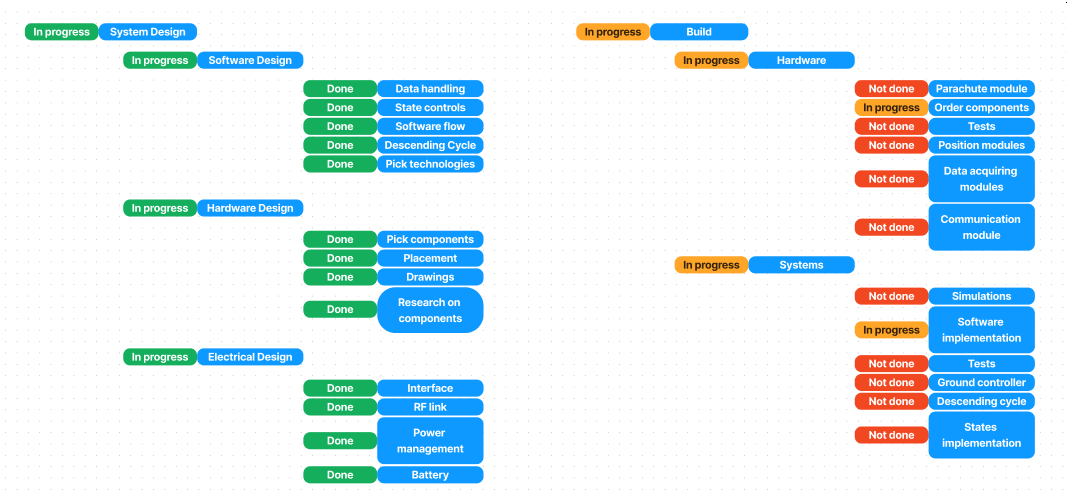
\includegraphics[width=15cm]{Tasks list.png}
\centering
\end{figure}

\subsection{Detailed project status}
\begin{enumerate}
    \item\textbf{Electrical design:}  {With a well design electrical scheme, that seeks power efficiency and increased runtime, we are ready to apply it to the actual satellite as soon as we have the necessary hardware components.}
    \item\textbf{Structural design:} {Using a Raspberry PI as the central board, for increased processing strength, caused a few problems about placement. Although our team managed to overcome this challenge by fitting all systems and components inside a can and proving ourselves that it is possible.}
    \item\textbf{Software design:} {Having C and Python as main programming languages, our software will be versatile and we have the power of adapting, as we will be able to have both, very low level programming such as C or Assembly integrated in C, but also high level programming trough Python if we need a fast and simple implementation. System designs are ready to be implemented, those including the descending cycle, state running system, and many more.}
    \item\textbf{Ground controller system:} {Our ground station is designed to monitor, control and communicate with the satellite central board, allowing us to make changes mid-flight and take emergency actions. These changes are possible due to the GCS having as equipment a laptop and the communication module.}
    \item\textbf{Power management system:} {Although solar panels came in the end that are not a valid option, our team managed to obtain a runtime of over 4 hours while acquiring data. The system is based on somewhat big batteries and a good efficiency from the electrical and software design.}
    \item\textbf{Communication system:} {The CS design allows the satellite to have a stable connection with GCS, using a GSM module with 4G network connection. This way we have a reliable connection because it is based on actual network and infrastructure.}
    \item\textbf{Hardware implementation:} {Having a complete list of specific components(list found at 4.2.1), necessary designs and a budget for the project, we will place an order for all components soon. Meanwhile components are on their way, our team is focused on research and finding new improvements.}
    \item\textbf{Software implementation:} {The software is already in progress, as building the foundation started. This means our team is focused on putting together a workspace, with necessary tools and technologies ready to work. Right after the workspace, the actual implementation will start.}
    \item\textbf{Outreach program:} {At the moment we are looking forward to gather some entertainment and educative content from our journey of implementing what we designed. When we are able to provide value(aka start implementation), we will start our social media engagement.}
\end{enumerate}





% 2nd section
\section{Introduction}
% Write the introduction text here

\subsection{Purpose of the mission}
\hspace{0.5cm} Overall goal is to help businesses pick a strategic placing for their entities, and to revolutionize GPS services with faster and more precise data. 

\subsection{Team organisation and roles}

\begin{enumerate}
\item \textbf{Team Name:} {ShuttleSat - shuttle is spaceship + sat is satellite, and we brought them together.}
\item \textbf{Team Composition:}
\begin{itemize}
\item[-] {Rares: Previous Experience → Hardware\&Embedded Google course \textbar\hspace{0cm} Background → pure sciences and maths \textbar\hspace{0cm} Interests → physics and mechanical engineering \textbar\hspace{0cm} Field of work within team → pick satellite's components, build the satellites, keeps track of available components, take care of components integrity, research and plan on physical components \textbar\hspace{0cm} Expected hours dedicated → 20-30.}
\item[-] {David: Background → electronics, signals and devices \textbar\hspace{0cm} Interests → electronic engineering \textbar\hspace{0cm} Field of work within team → R\&D, expertise in mission's area, data collect/analysis, timeline of data results, find and compare technical solutions, aerospace and electrical expertise \textbar\hspace{0cm} Expected hours dedicated → 20-30.}
\item[-] {Alex: Previous Experience → Project managing Innovation Labs mentorship \textbar\hspace{0cm} Background → analytical thinking and logical reasoning \textbar\hspace{0cm} Interests → team management and software engineering \textbar\hspace{0cm} Field of work within team → pick technologies, design and develop the software, meetings, initial ideas/information to start from maintain a developing plan, keep track of project directions, design/develop communication system \textbar\hspace{0cm} Expected hours dedicated → 20-30.}
\newline
\end{itemize}

\item \textbf{Team's Activity:} {Half meetings are online and half are physical, based on the expected length and progress review or the intended planification volume of the meet.}
\end{enumerate}

\subsection{Mission objectives}
\begin{enumerate}
    \item\textbf{Traffic measurement and mapping, for known congested areas, either entities identified as cars or humans.} {Secondary mission objective is to achieve an infrastructure capable of monitoring human and cars traffic. The infrastructure should be based on a single satellite that covers a single area at a time. We are looking forward to collect data such as: the number of entities inside the area and the flux of entities relative to time.}
    \item\textbf{Proving that the concept can be applied at a larger scale, such as a network of orbital satellites doing traffic measurements, is the target objective to call the launch successful.} {Main target is to successful capture stable and high quality pictures of the designated area. Smaller targets are to transmit this data to ground controller, and develop an innovative algorithm and AI in order to obtain 2 main variables: number of entities and their flux, within an area.}
    \item\textbf{We are expecting to find: majority of challenges, data to simulate actual implementation, costs and impact, infrastructure improvements.} {We are looking further to understand and list the majority of challenges that are faced when designing and building an orbiting satellite for current mission objective. Obtain the necessary data to run simulations of the cost to build and maintain a satellite network that measures and maps traffic, as well as it's impact and benefits. A flawless data transfer infrastructure is expected to be built trough the overcame challenges. Nonetheless we expect to improve our current skills and develop new ones, necessary for satellites development and engineering.}
    \item\textbf{Measure the values of CH4, CO2 and N2 and the quantity of entities inside a designated area.} {We are seeking to identify the \% of CH4, CO2 and N2 from the air with a precision of up to 98 at any altitude\% and the quantity of entities, in a targeted area with a precision of around 50\% at 300-700m for cars and 100-300m for humans. Also we are looking to test the transmission of this data, its capabilities and limitations, to the ground controller, continuously, until we fall under 100m of altitude. But the most important test will be the satellite as a whole, that every system work as expected and what improvements can be done for a successful infrastructure.}
\end{enumerate}


% 3rd section
\section{CanSat description / Payload description}
% Write the CanSat description text here for the CanSat challenge
% or the Payload escription text here for the Rocketry challenge

\subsection{Mission overview}
\hspace{0.5cm} We focus to \textbf{design} the satellite, its systems and perform a series of \textbf{simulations} and \textbf{theoretical tests}. Afterwards the mission will be carried out by \textbf{building} the CanSat, followed by several \textbf{tests, demonstrations} and \textbf{improvements}. The CanSat is set to be \textbf{launched} and \textbf{deployed} about 1km altitude, and to descend at about 10 meters per second, giving our \textbf{data systems} 80 seconds of straight data collecting time. Ground controller system, \textbf{processes} received data, throughout the entire time of data acquiring, and will provide \textbf{real-time statistics} from collected data.
\vspace{0.25cm}


\subsection{Mechanical / structural design}
% Here comes the text regarding the mechanical and structural design.
\begin{enumerate}
\item \textbf{Mechanical Design:} The CanSat is made of carbon fiber/ alluminum alloy because of their mechanical properties such as low weight, high durability and high tolerances in thermal expansion. The structure was designed to maintain a certain position while mid-air and to withstand the stress of launch and landing. It comes with a removable top and bottom to facilitate access inside. The components are attached to the structure with screws, nuts and mounts to assure stability during the mission.
\vspace{0.25cm}
\item \textbf{Components:} Components used for building the CanSat include: a main board, sensors, a video camera, a battery and a GPS module. The main board contains the microcontroller which collects the data from the sensors and sends it to the ground station via it’s communication module. The sensors include: a temperature sensor, a CH4 sensor, a N2 sensor, a CO2 sensor and an altimeter which measures both pressure and altitude. The GPS module registers the current position of the CanSat. The video camera takes frames of the surface below to be processed afterwards at the ground station. The battery provides power to the CanSat during flight. The list of components stands as it follows:

\begin{itemize}
\item \textbf{Microcontroller:} Raspberry PI Zero
\item \textbf{Temperature sensor:} sensor DS18B20
\item \textbf{CH4 sensor:} sensor MQ-4
\item \textbf{N2 sensor:} sensor MiCS-5524
\item \textbf{CO2 sensor:} sensor MQ-9
\item \textbf{Altimeter:} sensor BMP-388
\item \textbf{GPS Module:} GPS GY-NEO6MV2 module
\item \textbf{Communication module:} already integrated in main board
\item \textbf{Gyroscope:} sensor MPU6050
\item \textbf{Video Camera:} OV5647 video camera
\item \textbf{Rechargable battery:} portable power bank
\end{itemize}

\item \textbf{Placement:} The main board is attached to the top of the CanSat structure with the sensors located adjacent to it. The battery is attached to a side of the CanSat while the camera is attached to the opposite side of it. The structure was designed to maintain balance during flight, to minimize the weight and to provide space for the components and for further human intervention.
\vspace{0.25cm}
\item \textbf{Drawings:} This is a mechanical drawing of the CanSat structure in which we have emphasized on the placement of the major components.

\begin{figure}[hbt!]
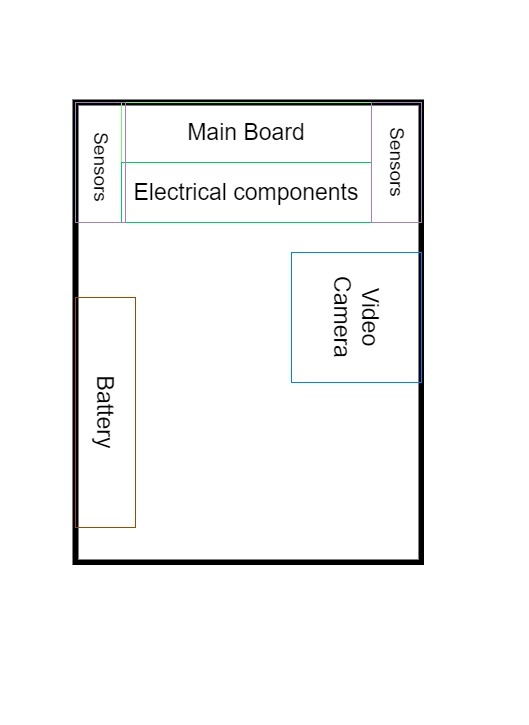
\includegraphics[width=8cm]{Component_placement}
\centering
\end{figure}

\item \textbf{Explanation:} The main board, Raspberry PI Zero acts as the data collector for the sensors and the camera, aswell as the data transmitter for the ground station. The sensor DS18B20 offers an accurate and fast measurement of the atmospheric temperature. MQ-4, MiCS-5524 and MQ-9 accomplish the main mission of the Payload, measurement of the quantity of atmospheric gasses. They all have a small power consumption and a very small error margin. Even though the BMP-388 is a Barometric Pressure sensor it can be used as a altimeter with a precision of $\pm$ 0.5 m. The GPS module GY-NEO6MV2 comes with an antenna which helps it receive the current position from the satellites and the MPU6050 sensor can be used as a 3 axis gyroscope. The OV5647 video camera is a standard Raspberry PI Camera with a small power consumption and a resoultion of 1080p which will be used to accomplish the secondary mission of the Payload, traffic measurement and mapping.

\end{enumerate}

\subsection{Electrical design}
% Here comes the text regarding the electrical design.
\begin{enumerate}
\item \textbf{Electrical Interface:}
\item \textbf{RF Link:}
\item \textbf{Power Budget:}
\item \textbf{Power Consumption and Duration:}
\item \textbf{Battery:} 

\begin{figure}[hbt!]
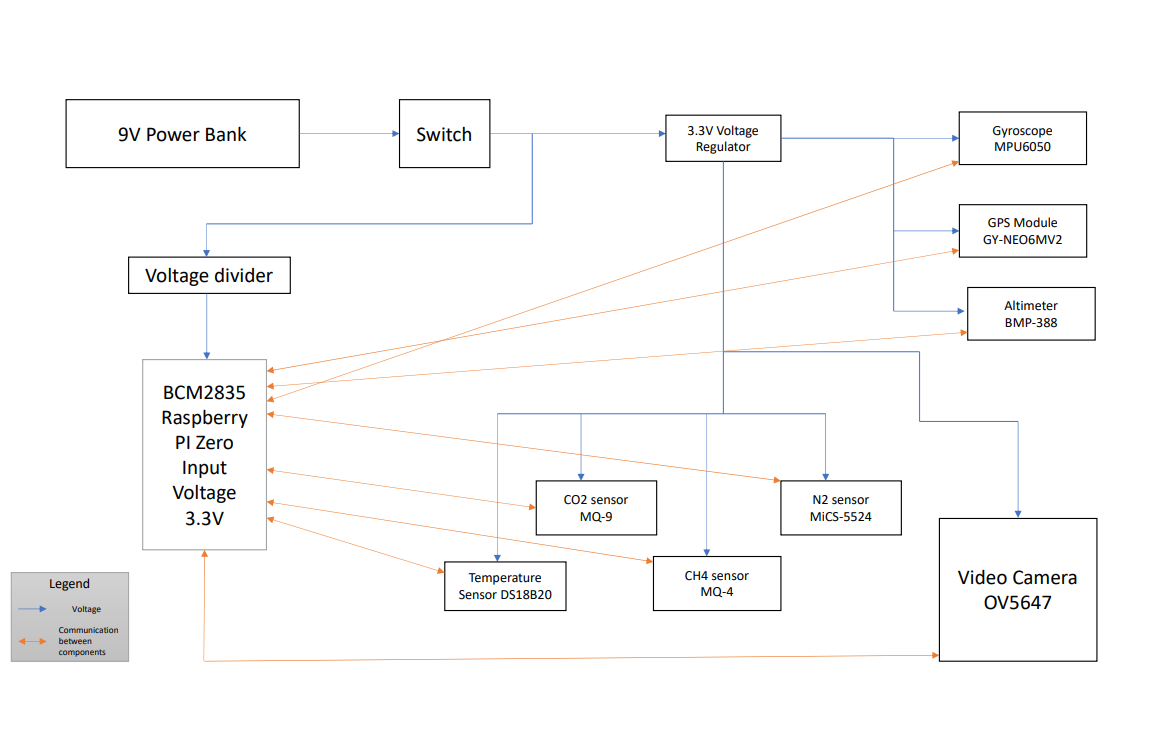
\includegraphics[width=15cm]{Schema_electrica}
\centering
\end{figure}
\end{enumerate}

\subsection{Software design}
\begin{enumerate}
\item \textbf{Introduction:} {The CanSat's robust software architecture is designed to seamlessly manage three key systems: the flying system, data acquisition, and data transmission. Powered by the Raspberry Pi Zero/Pico, our custom software ensures optimal energy efficiency and high-speed processing for precise control of the CanSat's mission.}
\item \textbf{Software flow overview:} {The software operates in predefined states, allowing the CanSat to adapt to various mission phases. In the event of any mid-flight issues, the system intelligently resumes from the last known state. For a detailed representation, refer to the Software Flow Diagram (SFD) atached below.}
\item \textbf{State based controls:} {Initiating from the boot phase, where the system verifies state integrity, the software progresses to standby, where all modules are idling. The subsequent ground test phase activates all modules at full power, testing their connections and integrity. The second phase commences with the launch, maintaining only the position modules, followed by ascent, where the parachute deployment system is engaged. The final stage, 'top/deploy,' marks the deployment of the chute. In the third phase, the position modules transition to idle, initiating the descending cycle. The last state, touchdown, signals the return of all modules to idle.}
\item \textbf{Data Handling:} {We anticipate a data volume ranging from 2Mb to 7Mb for images and over 10kb for sensor data per flight. The Raspberry Pi's non-volatile memory efficiently stores this data, ensuring data integrity throughout the mission. Real-time transmission to the ground station is facilitated through the communication system.}
\item \textbf{Programming Languages:} {C/C++ is employed for image data management, optimizing efficiency for handling larger datasets. Python, chosen for its versatility, manages sensor data efficiently, considering the smaller dataset size and lower processing requirements.}
\item \textbf{Conclusion:} {In conclusion, our software flow design not only ensures the reliability and adaptability of the CanSat but also facilitates efficient data management and transmission. This sophisticated architecture, coupled with the power of Raspberry Pi, positions our CanSat project for success in the upcoming challenge.}
\begin{figure}[h]
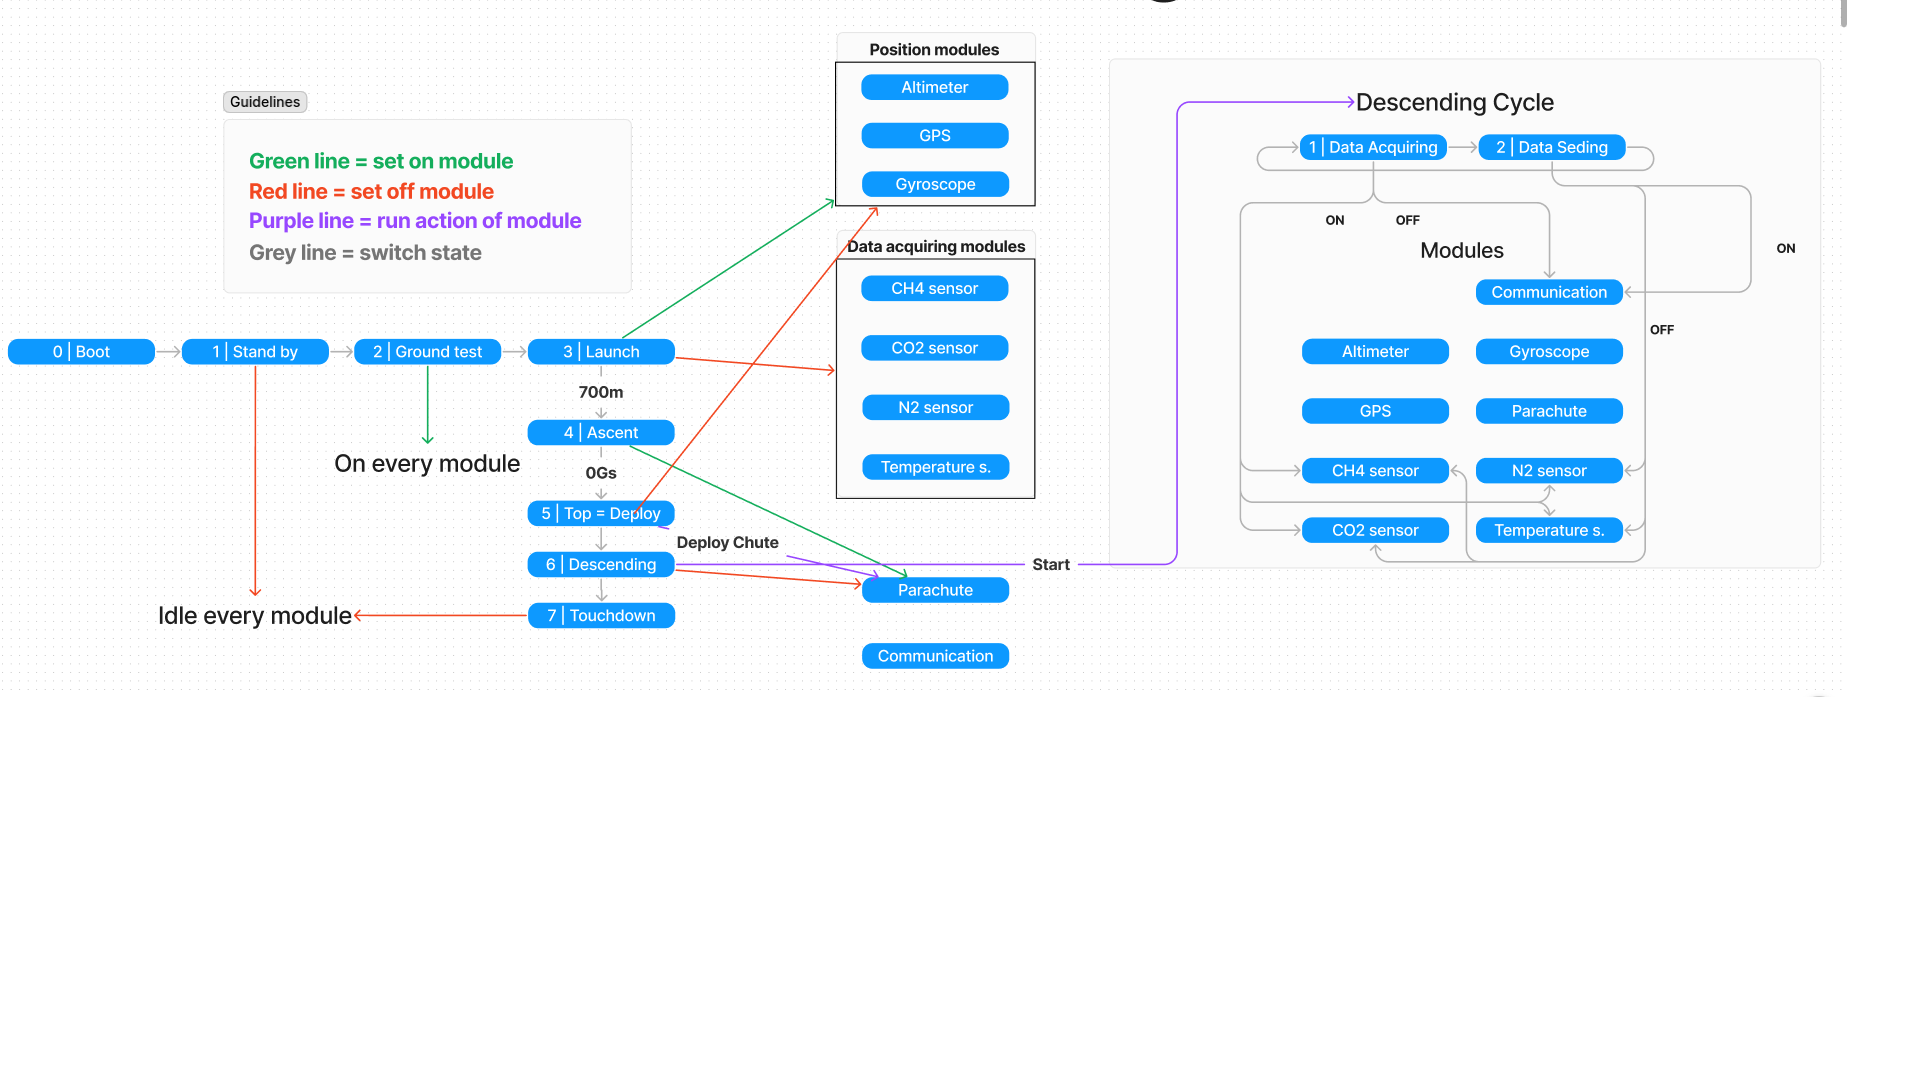
\includegraphics[width=19cm]{Software Diagram.png}
\centering
\end{figure}
\end{enumerate}
\begin{center}
\vspace{-4.5cm}
\centering
\textbf{S.F.D.}
\end{center}
\subsection{Recovery system}
% Here comes the text regarding the recovery system.
\begin{enumerate}
\item \textbf{Description:} The Recovery System of the CanSat is designed in order to be easy to make and to ensure a safe and controlled descent back to the ground station. It consists of a flat parachute with a drag coefficent of 0.77 and an area of 0.06 $m^2$, made with rip-stop fabric and attached to the CanSat via nylon cords. The parachute is deployed as soon as the CanSat is released from the rocket.
\vspace{0.25cm}
\item \textbf{Method of attachment:} The parachute is attached to the CanSat structure using a harness that is made of nylon fibres. The harness is connected to the structure itself with screws and PVC collars providing a stable attachment for the recovery system
\vspace{0.25cm}
\item \textbf{Picture:} Here is an indicative picture of how the parachute will look during the descent

\begin{figure}[hbt!]
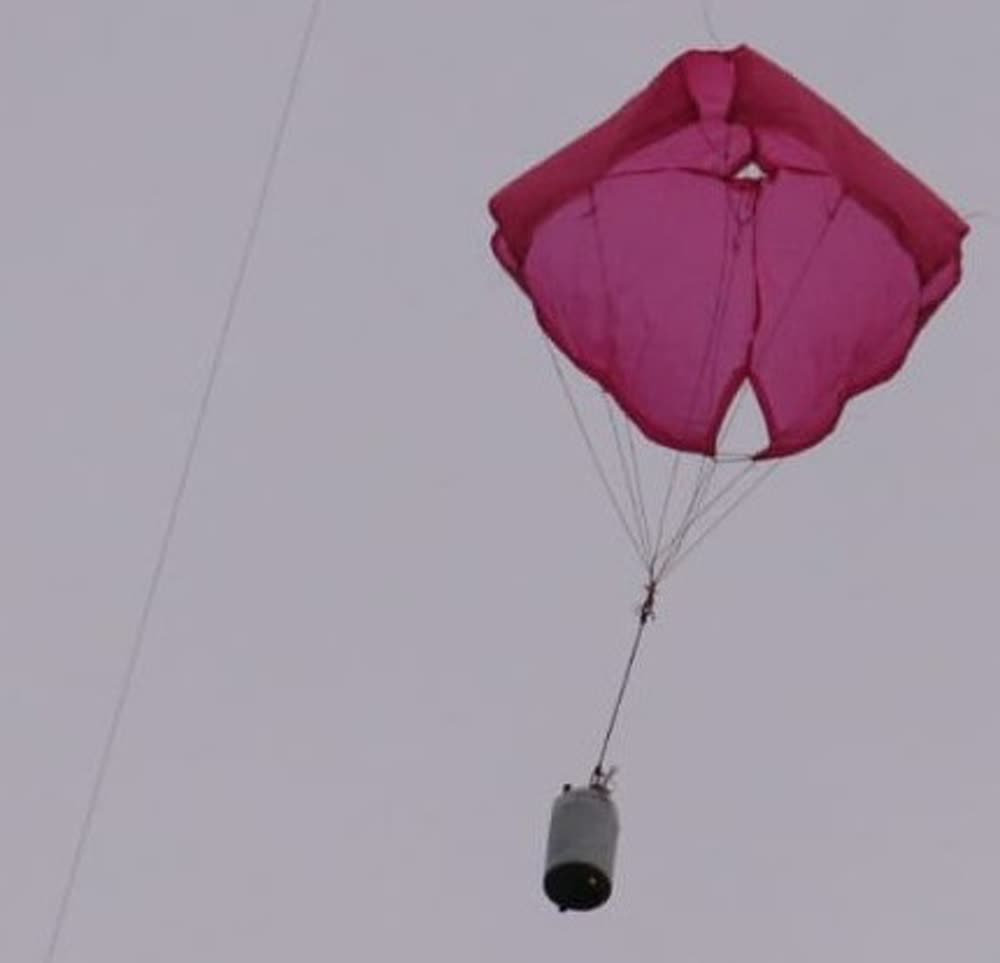
\includegraphics[width=5cm]{Parachute_example}
\centering
\end{figure}

\item \textbf{Expected flight time:} The CanSat's estimated flight time is around 10 minutes in which it reaches its maximum altitude and returns back to the ground station. After a short simulation, taking in consideration the characteristics of the parachute and of the Payload, the time for the descent is 100.7 seconds in perfect weather conditions and it reaches its maximum velocity of 10 m/s in 10 seconds. Here are the altitude and velocity variation graphs:

\begin{figure}[hbt!]
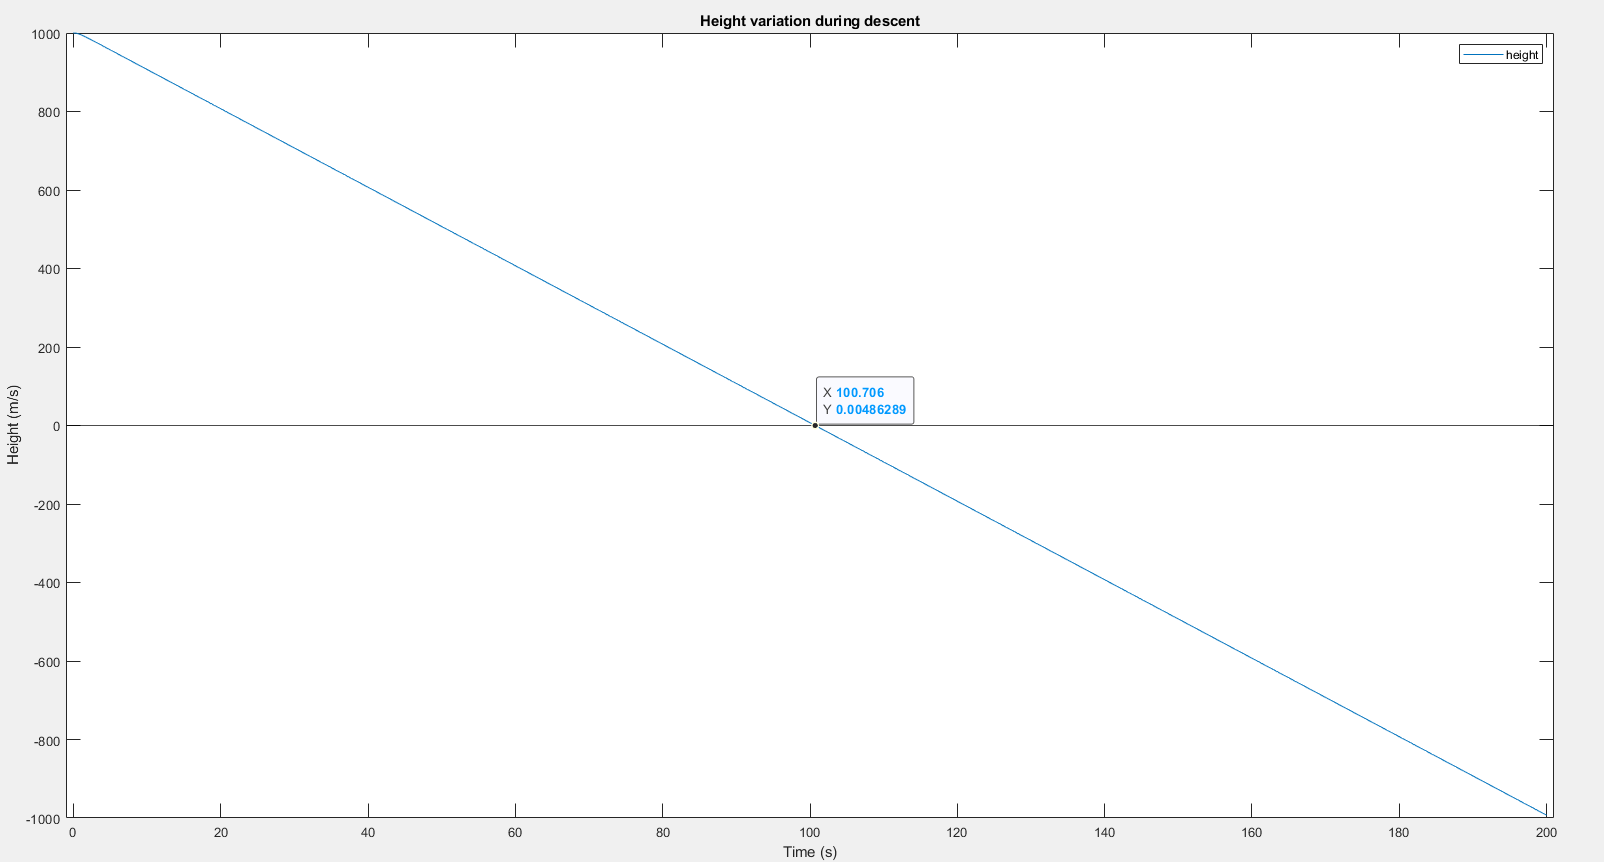
\includegraphics[width=15cm]{Height_variation}
\centering
\end{figure}

\begin{figure}[hbt!]
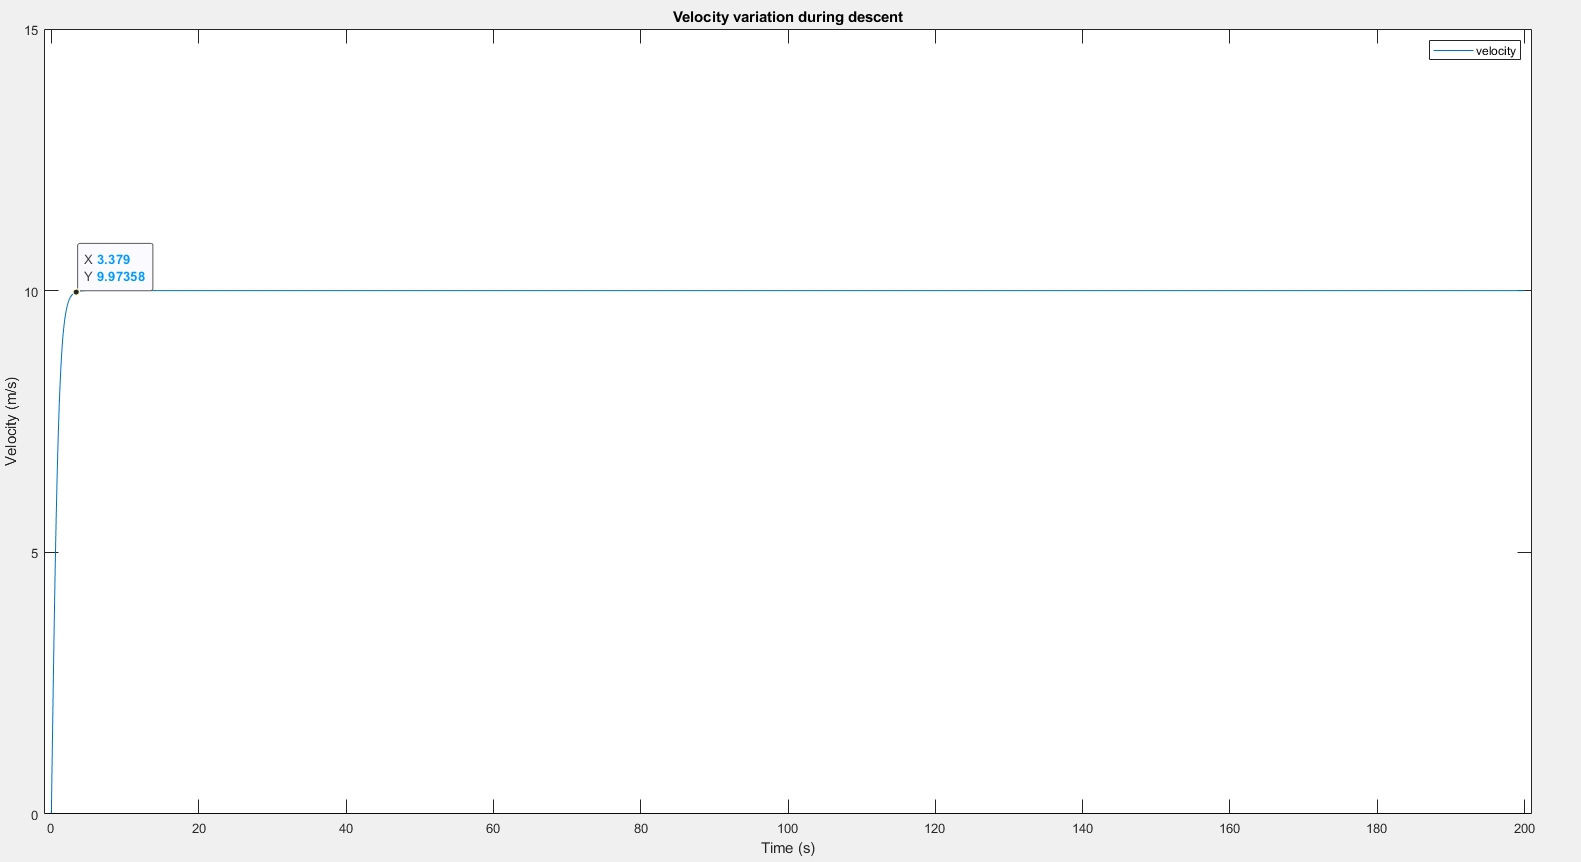
\includegraphics[width=15cm]{Velocity_variation}
\centering
\end{figure}

\end{enumerate}

\subsection{Ground support equipment}
\begin{enumerate}
\item \textbf{Introduction:} {Ground Support Equipment (GSE) consists of three main components: a laptop, an antenna, and a radio receiver. This system is vital for receiving and processing data transmitted by the CanSat during its mission.}
\item \textbf{Ground software design:} {The ground software design is segmented into two crucial parts. The backend is responsible for processing and storing data using advanced tools, including algorithms for image clarification and AI for comprehensive data analysis. Simple algorithms are also employed to process sensor data efficiently. On the other hand, the frontend is dedicated to presenting the processed data in a clear and human-understandable format, such as intuitive indicators like 'high level of traffic' or 'low level of traffic'.}
\item \textbf{Data handling and storage:} {All received and transmitted data are stored in binary format throughout the entire flight process. While binary data is utilized during the flight, a localized decoding process may be applied at the ground station for user experience and interface purposes.}
\item \textbf{Transmitter and data transmission:} {The transmitter, integral to the Raspberry Pi, facilitates data transmission and reception. Data is transfered trough a GSM module, and by operating a SIM card on the existing 4G network, our system minimizes interference with common signals in densely populated cities, such as Bucharest.}
\item \textbf{User friendly interface:} {The computer in our GSE will offer a user friendly interface, enabling operators to control various actions. This includes managing the 'descending cycle,' determining the focus of data gathering, toggling modules on/off, and additional functionalities designed to enhance mission control capabilities and reduce limitations.}
\item \textbf{Conclusion:} {In conclusion, our Ground Support Equipment is meticulously designed to receive, process, and interpret data from the CanSat during its mission, as well as send commands to the satellite and monitor every module and process by telemetry. The integration of advanced algorithms, binary data handling, and a user-friendly interface ensures the efficiency and effectiveness of our GSE in mission control.}
\end{enumerate}

% 4th section
\section{Project planning}
% Write about the project planning here

\subsection{Time schedule of the project preparation}
% Here comes the text regarding the time schedule.

\subsection{Resource estimation}
% Here comes the text regarding the resource estimation.

\subsubsection{Budget}
% Here comes the text regarding the budget.
\begin{center}
	\begin{tabular}{|c|c|}
		\hline
		  Component & Cost(RON) \\
		\hline
		  Microcontroller & 100\\
		  Temperature Sensor & 12\\
		  CH4 Sensor & 11\\
		  N2 Sensor & 80\\
		  CO2 Sensor & 15\\
		  Altimeter & 70\\
		  GPS Module & 50\\
		  Gyroscope & 17\\
		  Video Camera & 80\\
		  Rechargable Battery & 100\\
		  Structure & 200\\
		  Additional materials & 250\\
		  Personnel & 200\\
		  Launch site fees & 200\\
		\hline
		  Total Budget & 1385\\
		\hline
           \end{tabular}
\end{center}

\subsubsection{External support}
% Here comes the text regarding the external support.
\hspace{0.5cm} Our CanSat project, ShuttleSat, receives support just from the following departments:
\begin{itemize}
\item \textbf{University Politehnica Bucharest:} 
\begin{itemize}
\item[-] Professors from the Electronics and Telecomunications department are providing useful informations for the electric diagrams and components configurations
\item[-] Professors from the Computer Science department are offering advices in the choice of components and development of software
\end{itemize}
\end{itemize}

At the moment, the team lacks financial support for the purchase of components and also lacks support in the area of aerodynamics testing

\subsection{Test plan}
\begin{enumerate}
    \item\textbf{Simulations:} {In the beginning simulations will be our best friends, doing them will help us to find if a concept/implementation would work, and if not, why. Those include virtual simulations for electrical, software and hardware designs, and many more.}
    \item\textbf{Systems:} {First touch with actual testing will be by each system. While building either hardware or software, the systems will be tested independently. This will assure that the systems work, and if further problems are encountered at implementation we will know is probably from their communication rather than themselves.}
    \item\textbf{Prototype:} {Our team will test an iteration of the mission by using a prototype, all systems together, excluding actual conditions of the mission. This test will help us reinforce the connection between systems and their collaborative functionality.}
    \item\textbf{Real:} {The satellite will be part of several real tests, where we seek to find potential issues that can occur during flight and improvements. Some of these tests will be demonstrations for our public. This way we gather data and know what to change and expect in a real scenario and entertain our audience.}
\end{enumerate}

\subsection{Time management}
% Here comes the text regarding the time management.




% 5th section
\section{Data analysis and outreach}
% Here comes data analysis and outreach content.

\subsection{Data Analysis Plan}
% Here comes the text regarding the data analisys plan..
\hspace{0.5cm} The data analysis plan for the CanSat is designed to assure a clear understanding of the data it collects during the primary and secondary missions:
\begin{enumerate}
\item \textbf{Primary Mission:} Measurement of the quantities of atmospheric gasses: CH4, CO2 and N2 by using specific sensors mentioned above at different altitudes is the CanSat's primary mission. The data gathered by them will be directly sent to the microcontroller which further sends them to the ground station, then it will be analised and visually represented in a database.
\item \textbf{Secondary Mission:} As it was stated above, our CanSat's secondary mission is traffic measurement and mapping and finding a corellation between the traffic in a certain area and the density of the atmospheric gasses measured. The data gathered will consist of photos taken by the CanSat at different altitudes used for counting the entities at the ground such as cars and people.
\end {enumerate}
\hspace{0.5cm} In order for the data to be processed so it will offer us a great value, the following software will be used:
\begin{enumerate}
\item \textbf{Data acquisition software:} The Microcontroller uses a Unix interface which allows installing of different packages specific for each sensor to allow it to get the data from them. Also, the Microcontroller comes with a specific module for the video camera which allows it to get the image file obtained by the camera.
\item \textbf{Data  processing software:} The computer at the ground station will be using an algorithm for compressing the image and searching for key points of interest, especially for entities present in the image. Also, the data collected by the CanSat will be sent to a server in order to be downloaded in the ground station computer.
\item \textbf{Data visualisation software:} The data obtained will be represented visually in a program such as Matlab to quickly understand it and identify patterns and trends, especially in the case of traffic analysis and mapping which are key components of our secondary mission.
\item \textbf{Statistical analysis software:} The data obtained will be analised in a program such as Matlab to visualise if there is a connection between the density of the atmospheric gasses at different levels of altitude and the traffic in a certain area. It will consist in different types of charts, like cluster charts or regression charts that will help us determine if there truly is a corellation.
\end{enumerate}

\subsection{Outreach Program}
\begin{enumerate}
\item \textbf{Introduction:} {We embark on our CanSat challenge with a holistic outreach program aimed at building a thriving community around our project. Starting with a foundation on social media, we plan to engage and educate our audience through entertaining and informative content.}
\item \textbf{Social media strategy:} {As we progress and develop our first prototype, our social media presence will evolve from a '3 students hobby' to a platform for organic growth. We'll share behind-the-scenes moments, funny and documentary clips, fostering a connection with our audience.}
\item \textbf{Events and conferences:} {Participation in events and conferences will be a key element. These platforms will serve as avenues to showcase our prototype to potential investors, clients, and sponsors. Simultaneously, we'll leverage these opportunities to educate the community, sharing insights into the challenges we face and our innovative problem-solving approaches.}
\item \textbf{Demonstrations:} {To create a buzz and increase awareness, we'll organize engaging demonstrations, while redoing key tests. Leveraging various channels like flyers, posters, our students league (LSAC), and social media, we'll promote these events with a touch of entertainment, ensuring they become memorable ('Falling satellite at 3:00PM from the rectory building – watch out for your head').}
\item \textbf{Hosting events:} {As we grow, hosting events will become a reality. This opens doors for collaborations and sponsorship opportunities. Social media channels will transition into platforms for event promotion, sharing event-based photos, and connecting with our community.}
\item \textbf{Website utilization:} {The website will be a central hub for technical updates, showcasing our accomplishments and outlining our future goals. Real-time data from our satellite, live camera feeds, and effective SEO strategies will enhance the site's value.}
\item \textbf{Financial resources and team development:} {Further we are looking to access financial resources which will be the turning point. We'll invest in team development, providing training for current members and welcoming new talents. This infusion of funds will elevate our social media, marketing, and event strategies, positioning us as a new contender in the industry.}
\item \textbf{Conclusion:} {In summary, our outreach program is designed to create a dynamic and engaged community around our CanSat project. From social media to events, collaborations, and a robust website, we aim to not only excel in the CanSat challenge but also leave a lasting impact on our community and industry partners.}
\end{enumerate}



% 6th section
\section{Conclusion}
% Here comes the conclusion content.

\subsection{Summary of the CDR}
% Here comes the summary for the CDR
\hspace{0.5cm} To sumarise everything mentioned above, the "ShuttleSat" CanSat is designed to fulfill two missions: the quantity measurement of the atmospheric gasses and traffic management and mapping, and to find a connection between them. Even though this may not be accomplished with such a small scale project, we have high hopes regarding the value of the data that will be collected. We look forward to achieving a recognition of people in the pictures taken at the altitudes of under 300m, aswell as recognition of cars at under 700m and a very precise measurement of the density of gasses such as CH4, CO2 and N2.
\newline

At the moment, we are aware of the fact that the structure of the CanSat and the details of the missions are subject to change since there are certain conditions or risks we have not taken into consideration. Though, as it stands right now, we envision that the current design will be able to sustain bad weather such as a windy or a cloudy weather and that the components and software that we thought of are going to be able to collect and process the data we want. If not, we will make the necessary adjustments such as changing the components or the structure and materials of the CanSat itself or we will look towards other pieces of software that will be more efficient in order to achieve our objectives.



\subsection{Recommendations for next steps}
% Here comnes the recomandations for the next phase/steps
\hspace{0.5cm} As we are preparing for the next phase, we are starting to take in consideration emergency measures to avoid future problems such as:
\begin{enumerate}
\item Expanding our component list to have alternatives in case of one being insufficient for realising its purpose.
\item Looking for multiple ways of funding our project to avoid not having enough funds to buy the necessary materials.
\item Finding a way to stabilise the CanSat during its descent to assure that the photos will be clear and easy to analise.
\item Finding alternatives for the outreach strategy in case of the feedback not being as good as expected.
\end{enumerate}

\end{document}
